\documentclass[twoside]{article}

% Packages required by doxygen
\usepackage{fixltx2e}
\usepackage{calc}
\usepackage{doxygen}
\usepackage{graphicx}
\usepackage[utf8]{inputenc}
\usepackage{makeidx}
\usepackage{multicol}
\usepackage{multirow}
\PassOptionsToPackage{warn}{textcomp}
\usepackage{textcomp}
\usepackage[nointegrals]{wasysym}
\usepackage[table]{xcolor}

% Font selection
\usepackage[T1]{fontenc}
\usepackage{mathptmx}
\usepackage[scaled=.90]{helvet}
\usepackage{courier}
\usepackage{amssymb}
\usepackage{sectsty}
\renewcommand{\familydefault}{\sfdefault}
\allsectionsfont{%
  \fontseries{bc}\selectfont%
  \color{darkgray}%
}
\renewcommand{\DoxyLabelFont}{%
  \fontseries{bc}\selectfont%
  \color{darkgray}%
}
\newcommand{\+}{\discretionary{\mbox{\scriptsize$\hookleftarrow$}}{}{}}

% Page & text layout
\usepackage[screen]{geometry}
\tolerance=750
\hfuzz=15pt
\hbadness=750
\setlength{\emergencystretch}{15pt}
\setlength{\parindent}{0cm}
\setlength{\parskip}{0.2cm}
\makeatletter
\renewcommand{\paragraph}{%
  \@startsection{paragraph}{4}{0ex}{-1.0ex}{1.0ex}{%
    \normalfont\normalsize\bfseries\SS@parafont%
  }%
}
\renewcommand{\subparagraph}{%
  \@startsection{subparagraph}{5}{0ex}{-1.0ex}{1.0ex}{%
    \normalfont\normalsize\bfseries\SS@subparafont%
  }%
}
\makeatother

% Headers & footers
\usepackage{fancyhdr}
\pagestyle{fancyplain}
\fancyhead[LE]{\fancyplain{}{\bfseries\thepage}}
\fancyhead[CE]{\fancyplain{}{}}
\fancyhead[RE]{\fancyplain{}{\bfseries\leftmark}}
\fancyhead[LO]{\fancyplain{}{\bfseries\rightmark}}
\fancyhead[CO]{\fancyplain{}{}}
\fancyhead[RO]{\fancyplain{}{\bfseries\thepage}}
\fancyfoot[LE]{\fancyplain{}{}}
\fancyfoot[CE]{\fancyplain{}{}}
\fancyfoot[RE]{\fancyplain{}{\bfseries\scriptsize Generated on Fri Nov 17 2017 07\+:11\+:56 by Doxygen }}
\fancyfoot[LO]{\fancyplain{}{\bfseries\scriptsize Generated on Fri Nov 17 2017 07\+:11\+:56 by Doxygen }}
\fancyfoot[CO]{\fancyplain{}{}}
\fancyfoot[RO]{\fancyplain{}{}}
\renewcommand{\footrulewidth}{0.4pt}
\renewcommand{\sectionmark}[1]{%
  \markright{\thesection\ #1}%
}

% Indices & bibliography
\usepackage{natbib}
\usepackage[titles]{tocloft}
\setcounter{tocdepth}{3}
\setcounter{secnumdepth}{5}
\makeindex

% Packages requested by user
\usepackage{titlesec}

% Hyperlinks (required, but should be loaded last)
\usepackage{ifpdf}
\ifpdf
  \usepackage[pdftex,pagebackref=true]{hyperref}
\else
  \usepackage[ps2pdf,pagebackref=true]{hyperref}
\fi
\hypersetup{%
  colorlinks=true,%
  linkcolor=blue,%
  citecolor=blue,%
  unicode%
}

% Custom commands
\newcommand{\clearemptydoublepage}{%
  \newpage{\pagestyle{empty}\cleardoublepage}%
}


\newcommand{\sectionbreak}{\clearpage}

\begin{document}

% Titlepage & ToC
\hypersetup{pageanchor=false,
             bookmarks=true,
             bookmarksnumbered=true,
             pdfencoding=unicode
            }
\pagenumbering{roman}
\begin{titlepage}
\vspace*{7cm}
\begin{center}%
{\Large Reference Manual}\\
\vspace*{1cm}
{\large Generated by Doxygen 1.8.8}\\
\vspace*{0.5cm}
{\small Fri Nov 17 2017 07:11:56}\\
\end{center}
\end{titlepage}
\tableofcontents
\pagenumbering{arabic}
\hypersetup{pageanchor=true}

%--- Begin generated contents ---
\section{Telegraph\+:\+:decode}
\label{Telegraph_1_1decode}
\hypertarget{Telegraph_1_1decode}{}
decodes morse code into english text


\begin{DoxyParams}[1]{Parameters}
\mbox{\tt in,out}  & {\em text} & A char array holding inputted or translated english text \\
\hline
\mbox{\tt in,out}  & {\em morse} & A char array holding inputted or translated morse code \\
\hline
\end{DoxyParams}
\begin{DoxyReturn}{Returns}
void 
\end{DoxyReturn}

\section{Telegraph\+:encode}
\label{Telegraph_1encode}
\hypertarget{Telegraph_1encode}{}
encodes an english message into morse code


\begin{DoxyParams}[1]{Parameters}
\mbox{\tt in,out}  & {\em text} & A char array holding inputted or translated english text \\
\hline
\mbox{\tt in,out}  & {\em morse} & A char array holding inputted or translated morse code \\
\hline
\end{DoxyParams}
\begin{DoxyReturn}{Returns}
void 
\end{DoxyReturn}

\section{Morse\+Code}
\label{MorseCode}
\hypertarget{MorseCode}{}
A struct holding letters of the alphabet along with numbers and special characters. Each symbol is associated with a morse code sequence,a max of 7 '.'s or '-\/'s total can be held in the sequence. 
\section{T\+N\+O\+D\+E}
\label{TNODE}
\hypertarget{TNODE}{}
A tree node to be used in creation of the binary tree. Used in conjunction with the open() function, when creating the tree, a tree node is made with '$\ast$' as a default symbol and no child nodes. The symbol is overwritten if the sequence ends at that tree node and child nodes are created if the sequence forces a node to be made there. 
\section{Class\+: Telegraph}
\label{Class_1_01Telegraph}
\hypertarget{Class_1_01Telegraph}{}
A class holding a table of size 40 consisting of symbols and their morse code equivalents. A root node is created automatically for creation of the binary tree. A Destroy\+Tree() function exists for the closing process of the binary tree. The class has open() and close() functions for maintaining the morse code binary tree. The class also holds encode() and decode() functions for english to morse translations and vice versa. 
\section{Telegraph\+:\+:open()}
\label{Telegraph_1_1open_07_08}
\hypertarget{Telegraph_1_1open_07_08}{}
Creates and opens a binary tree holding english symbols and their morse code equivalents

A table holding english symbols and their morse code equivalent is read. For each symbol, the morse code sequence is read and a node pointer points through the nodes depending on the sequence, creating nodes if they don't exist. If a '.' is read, it moves into the left child node of the root. If a '-\/' is read, it moves into the right child node of the root. This keeps going until the end of the sequence. For example, '.--' would cause the node pointer to point to the left child node of the root, then the right child node of the node it was pointing to, and then the left child node again of the node it was pointing to. If the nodes didn't exist, they would be created. At the end of the sequence, the symbol associated with it is stored in the node and the node pointer goes back to root, restarting the process until the table is finished. 
\section{Telegraph\+:\+:Destroy\+Tree/\+Telegraph\+:\+:close()}
\label{Telegraph_1_1DestroyTree_2Telegraph_1_1close_07_08}
\hypertarget{Telegraph_1_1DestroyTree_2Telegraph_1_1close_07_08}{}
Traverses the binary tree, deleting each node until finally deleting the root node itself

The root node is passed in and begins the deletion process. The close function calls Destroy\+Tree, a recursive function that will traverse the tree until it hits the end of both sides. Once that happens, the nodes are deleted until it reaches root. Root is then deleted, triggering the base case where a node does not exist, ending the function


\begin{DoxyParams}[1]{Parameters}
\mbox{\tt in}  & {\em $\ast$node} & The root node of the binary tree \\
\hline
\end{DoxyParams}
\begin{DoxyReturn}{Returns}
void 
\end{DoxyReturn}

\section{Specification}
\label{Specification}
\hypertarget{Specification}{}
This is the English-\/\+Italian Dictionary program. The user can input an English word and the program will provide translation of the word. The current file the program uses to translate is and English to Italian Dictionary If the word that user enters is not in the program the the user can add the word into the dictionary by following the instructions given by the program.

Freatures\+:

1) The instructures are clear and concise to understand.

2) The ability to add words into the dictionary/program for later use.

3) Operator overlaoding to improve effiecncy of program. 
\section{Analysis}
\label{Analysis}
\hypertarget{Analysis}{}
When the user goes to the html page the program is already running. Here the user will be greeted by 6 options to select from. 5 of these options are sorting algorithms the other one is an option to see the times it takes for them to sort. When a sort is selected the page will load the name of the sort and then all the sorted info below it. Th fastest sort was quick sort which took less than a second. The slowest was bubble which varied from 40 seconds to 3 minutes. 
\section{Design}
\label{Design}
\hypertarget{Design}{}
Html was what we used to create the U\+I for this lab. T\+He translation program however was done in C++. We implemented a binary tree which basically allows us to store elements that can reference elements lower than it. Like tree -\/$>$ branches -\/$>$ twigs -\/$>$ leaves. The idea is that only an element of lower value can be stored in bottom of another element and lower is on the left and greater on the right. So in our lab a . was considered lower and a -\/ was conidered higher. This allowed us to reference letters within the tree very quickly. 
\section{Test\+: Morse 1}
\label{Test_1_01Morse_011}
\hypertarget{Test_1_01Morse_011}{}

\begin{DoxyImage}
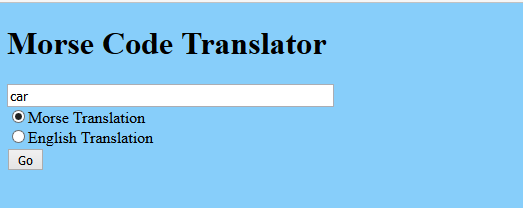
\includegraphics[width=15cm]{morse1.PNG}
\caption{Morse code to be decoded}
\end{DoxyImage}
 
\section{Test\+: Morse 2}
\label{Test_1_01Morse_012}
\hypertarget{Test_1_01Morse_012}{}

\begin{DoxyImage}
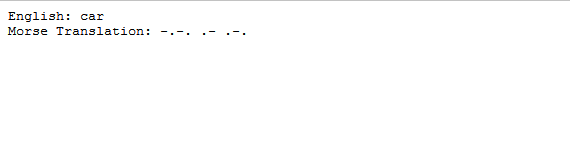
\includegraphics[width=15cm]{morse2.PNG}
\caption{Morse code decoded}
\end{DoxyImage}
 
\section{Test\+: Morse Verified}
\label{Test_1_01Morse_01Verified}
\hypertarget{Test_1_01Morse_01Verified}{}

\begin{DoxyImage}
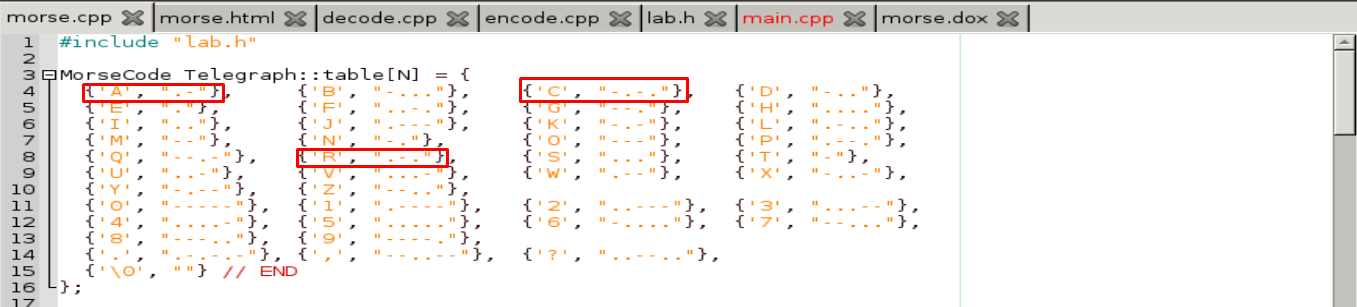
\includegraphics[width=15cm]{morse3.png}
\caption{Morse code verified}
\end{DoxyImage}
 
\section{Test\+: English 1}
\label{Test_1_01English_011}
\hypertarget{Test_1_01English_011}{}

\begin{DoxyImage}
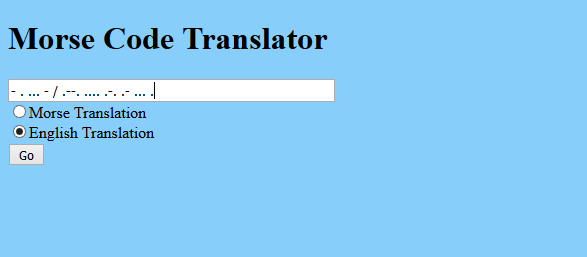
\includegraphics[width=15cm]{english1.png}
\caption{English text to be encoded}
\end{DoxyImage}
 
\section{Test\+: English 2}
\label{Test_1_01English_012}
\hypertarget{Test_1_01English_012}{}

\begin{DoxyImage}
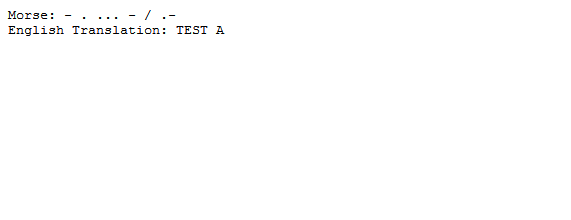
\includegraphics[width=15cm]{english2.png}
\caption{English text encoded}
\end{DoxyImage}
 
\section{Test\+: English Verified}
\label{Test_1_01English_01Verified}
\hypertarget{Test_1_01English_01Verified}{}

\begin{DoxyImage}
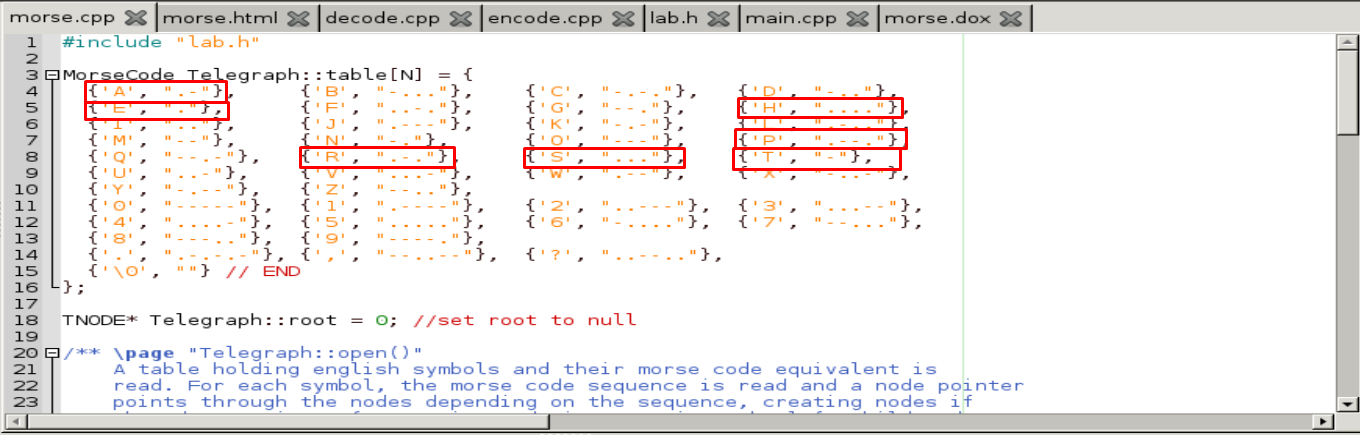
\includegraphics[width=15cm]{english3.png}
\caption{English text verified}
\end{DoxyImage}
 
\section{Morse Binary Tree}
\label{Morse_01Binary_01Tree}
\hypertarget{Morse_01Binary_01Tree}{}

\begin{DoxyImage}
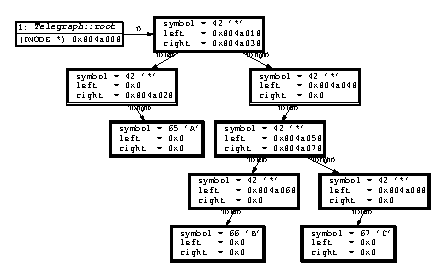
\includegraphics[width=15cm]{morseTree}
\caption{Morse Tree}
\end{DoxyImage}
 
\section{H\+T\+M\+L}
\label{HTML}
\hypertarget{HTML}{}

\begin{DoxyVerbInclude}
<!DOCTYPE html PUBLIC "-//W3C//DTD XHTML 1.0 Strict//EN" "http://www.w3.org/TR/xhtml1/DTD/xhtml1-strict.dtd">
<!-- saved from url=(0043)http://localhost:8080/cs124/lab6/morse.html -->
<html xmlns="http://www.w3.org/1999/xhtml" xml:lang="en" lang="en" wtx-context="6D7991A1-0A29-456F-A1AE-A3E37871556A"><head><meta http-equiv="Content-Type" content="text/html; charset=UTF-8">
	<title>CS 124 Lab 6 - MORSE CODE TRANSLATOR</title>
	
	<meta name="generator" content="Geany 1.24.1">
</head>

<body bgcolor="#87CEFA">
   <h1>Morse Code Translator</h1> 
   <form action="http://localhost:8080/cgi-bin/morse" wtx-context="3E5B8EA5-7244-4FCB-B3CB-CF9880D40BE8">
       <input type="text" name="e" size="50">
       <br>
       <input type="radio" name="o" value="morse">Morse Translation
       <br>
       <input type="radio" name="o" value="english">English Translation
       <br>
       <input type="submit" value="Go">
   </form>
   <!--img src="/images/graph.png"-->



</body></html>
\end{DoxyVerbInclude}
 
\section{Class Index}
\subsection{Class List}
Here are the classes, structs, unions and interfaces with brief descriptions\+:\begin{DoxyCompactList}
\item\contentsline{section}{\hyperlink{structFRAGMENT}{F\+R\+A\+G\+M\+E\+N\+T} }{\pageref{structFRAGMENT}}{}
\item\contentsline{section}{\hyperlink{structMUSICELMT}{M\+U\+S\+I\+C\+E\+L\+M\+T} }{\pageref{structMUSICELMT}}{}
\item\contentsline{section}{\hyperlink{structNOTE}{N\+O\+T\+E} }{\pageref{structNOTE}}{}
\item\contentsline{section}{\hyperlink{structSTACK}{S\+T\+A\+C\+K} }{\pageref{structSTACK}}{}
\end{DoxyCompactList}

\section{File Index}
\subsection{File List}
Here is a list of all files with brief descriptions\+:\begin{DoxyCompactList}
\item\contentsline{section}{\hyperlink{addWords_8cpp}{add\+Words.\+cpp} }{\pageref{addWords_8cpp}}{}
\item\contentsline{section}{\hyperlink{foundWord_8cpp}{found\+Word.\+cpp} }{\pageref{foundWord_8cpp}}{}
\item\contentsline{section}{\hyperlink{lab_8cpp}{lab.\+cpp} }{\pageref{lab_8cpp}}{}
\item\contentsline{section}{\hyperlink{lab_8h}{lab.\+h} }{\pageref{lab_8h}}{}
\item\contentsline{section}{\hyperlink{loadDictionary_8cpp}{load\+Dictionary.\+cpp} }{\pageref{loadDictionary_8cpp}}{}
\item\contentsline{section}{\hyperlink{main_8cpp}{main.\+cpp} }{\pageref{main_8cpp}}{}
\end{DoxyCompactList}

\section{Class Documentation}
\hypertarget{structMorseCode}{\subsection{Morse\+Code Struct Reference}
\label{structMorseCode}\index{Morse\+Code@{Morse\+Code}}
}


{\ttfamily \#include $<$lab.\+h$>$}

\subsubsection*{Public Types}
\begin{DoxyCompactItemize}
\item 
enum \{ \hyperlink{structMorseCode_ab70bfb3505458b9ca361321710a3bf4ea255fc4372695bc3e775c82488bfc2dac}{N} =7
 \}
\end{DoxyCompactItemize}
\subsubsection*{Public Attributes}
\begin{DoxyCompactItemize}
\item 
char \hyperlink{structMorseCode_a15f3e521a3db80ec2f44a9c42b5cb949}{symbol}
\item 
char \hyperlink{structMorseCode_aeb273082df944b0bc60d1388f215b1b7}{code} \mbox{[}\hyperlink{structMorseCode_ab70bfb3505458b9ca361321710a3bf4ea255fc4372695bc3e775c82488bfc2dac}{N}\mbox{]}
\end{DoxyCompactItemize}


\subsubsection{Member Enumeration Documentation}
\hypertarget{structMorseCode_ab70bfb3505458b9ca361321710a3bf4e}{\paragraph[{anonymous enum}]{\setlength{\rightskip}{0pt plus 5cm}anonymous enum}}\label{structMorseCode_ab70bfb3505458b9ca361321710a3bf4e}
\begin{Desc}
\item[Enumerator]\par
\begin{description}
\index{N@{N}!Morse\+Code@{Morse\+Code}}\index{Morse\+Code@{Morse\+Code}!N@{N}}\item[{\em 
\hypertarget{structMorseCode_ab70bfb3505458b9ca361321710a3bf4ea255fc4372695bc3e775c82488bfc2dac}{N}\label{structMorseCode_ab70bfb3505458b9ca361321710a3bf4ea255fc4372695bc3e775c82488bfc2dac}
}]\end{description}
\end{Desc}

\begin{DoxyCode}
14 \{\hyperlink{structMorseCode_ab70bfb3505458b9ca361321710a3bf4ea255fc4372695bc3e775c82488bfc2dac}{N}=7\};
\end{DoxyCode}


\subsubsection{Member Data Documentation}
\hypertarget{structMorseCode_aeb273082df944b0bc60d1388f215b1b7}{\index{Morse\+Code@{Morse\+Code}!code@{code}}
\index{code@{code}!Morse\+Code@{Morse\+Code}}
\paragraph[{code}]{\setlength{\rightskip}{0pt plus 5cm}char Morse\+Code\+::code\mbox{[}{\bf N}\mbox{]}}}\label{structMorseCode_aeb273082df944b0bc60d1388f215b1b7}
\hypertarget{structMorseCode_a15f3e521a3db80ec2f44a9c42b5cb949}{\index{Morse\+Code@{Morse\+Code}!symbol@{symbol}}
\index{symbol@{symbol}!Morse\+Code@{Morse\+Code}}
\paragraph[{symbol}]{\setlength{\rightskip}{0pt plus 5cm}char Morse\+Code\+::symbol}}\label{structMorseCode_a15f3e521a3db80ec2f44a9c42b5cb949}


The documentation for this struct was generated from the following file\+:\begin{DoxyCompactItemize}
\item 
\hyperlink{lab_8h}{lab.\+h}\end{DoxyCompactItemize}

\hypertarget{classTelegraph}{\subsection{Telegraph Class Reference}
\label{classTelegraph}\index{Telegraph@{Telegraph}}
}


{\ttfamily \#include $<$lab.\+h$>$}

\subsubsection*{Public Member Functions}
\begin{DoxyCompactItemize}
\item 
void \hyperlink{classTelegraph_ac076aaff18187105bbc553302cf630d5}{encode} (char text\mbox{[}$\,$\mbox{]}, char morse\mbox{[}$\,$\mbox{]})
\item 
void \hyperlink{classTelegraph_a131e9c2acc739501496b9b7f48e833aa}{decode} (char morse\mbox{[}$\,$\mbox{]}, char text\mbox{[}$\,$\mbox{]})
\end{DoxyCompactItemize}
\subsubsection*{Static Public Member Functions}
\begin{DoxyCompactItemize}
\item 
static void \hyperlink{classTelegraph_a2ace7d6ba4d3742dbcc57d6a36a13b54}{open} ()
\item 
static void \hyperlink{classTelegraph_a5a49093b588a538d53449aba1e66f44c}{close} ()
\end{DoxyCompactItemize}


\subsubsection{Member Function Documentation}
\hypertarget{classTelegraph_a5a49093b588a538d53449aba1e66f44c}{\index{Telegraph@{Telegraph}!close@{close}}
\index{close@{close}!Telegraph@{Telegraph}}
\paragraph[{close}]{\setlength{\rightskip}{0pt plus 5cm}static void Telegraph\+::close (
\begin{DoxyParamCaption}
{}
\end{DoxyParamCaption}
)\hspace{0.3cm}{\ttfamily [inline]}, {\ttfamily [static]}}}\label{classTelegraph_a5a49093b588a538d53449aba1e66f44c}

\begin{DoxyCode}
56 \{ DestroyTree(root); \}
\end{DoxyCode}
\hypertarget{classTelegraph_a131e9c2acc739501496b9b7f48e833aa}{\index{Telegraph@{Telegraph}!decode@{decode}}
\index{decode@{decode}!Telegraph@{Telegraph}}
\paragraph[{decode}]{\setlength{\rightskip}{0pt plus 5cm}void Telegraph\+::decode (
\begin{DoxyParamCaption}
\item[{char}]{morse\mbox{[}$\,$\mbox{]}, }
\item[{char}]{text\mbox{[}$\,$\mbox{]}}
\end{DoxyParamCaption}
)}}\label{classTelegraph_a131e9c2acc739501496b9b7f48e833aa}

\begin{DoxyCode}
10 \{
11     \textcolor{keywordtype}{char} *dd;
12     \textcolor{keywordtype}{int} count = 0;
13     \hyperlink{structTNODE}{TNODE} *node;
14     
15     node = root;
16     \textcolor{keywordflow}{for}(dd = morse; *dd; dd++) \{
17         \textcolor{keywordflow}{if}(*dd == \textcolor{charliteral}{'.'}) 
18             node = node->\hyperlink{structTNODE_ac8548d0ee2d54b914e0e07ab35375dba}{left};
19         \textcolor{keywordflow}{else} \textcolor{keywordflow}{if}(*dd == \textcolor{charliteral}{'-'})
20             node = node->\hyperlink{structTNODE_a4e135d9137519b2a4b89dbccb55ae967}{right};
21         \textcolor{keywordflow}{else} \textcolor{keywordflow}{if}(*dd == \textcolor{charliteral}{'/'}) \{
22             node->\hyperlink{structTNODE_a436db20d992c4227b8482603b4f76712}{symbol} = \textcolor{charliteral}{' '};
23         \}   
24         \textcolor{keywordflow}{else} \{
25             text[count] = node->\hyperlink{structTNODE_a436db20d992c4227b8482603b4f76712}{symbol};
26             node = root;
27             count++;
28         \}
29     \}
30 \}
\end{DoxyCode}
\hypertarget{classTelegraph_ac076aaff18187105bbc553302cf630d5}{\index{Telegraph@{Telegraph}!encode@{encode}}
\index{encode@{encode}!Telegraph@{Telegraph}}
\paragraph[{encode}]{\setlength{\rightskip}{0pt plus 5cm}void Telegraph\+::encode (
\begin{DoxyParamCaption}
\item[{char}]{text\mbox{[}$\,$\mbox{]}, }
\item[{char}]{morse\mbox{[}$\,$\mbox{]}}
\end{DoxyParamCaption}
)}}\label{classTelegraph_ac076aaff18187105bbc553302cf630d5}

\begin{DoxyCode}
10 \{
11     \textcolor{keywordtype}{int} i;
12     \textcolor{keywordtype}{char} c, *t, *dd; \textcolor{comment}{// t points to text}
13                      \textcolor{comment}{// dd points to a string of dots and dashes}
14     \textcolor{keywordflow}{for}(t = text; *t; t++)
15     \{
16         
17         c = toupper(*t);
18         
19         \textcolor{comment}{// If space, add a space to the morse string:}
20         \textcolor{keywordflow}{if}(c == \textcolor{charliteral}{' '}) \{
21             *morse++ = \textcolor{charliteral}{'/'};
22             *morse++ = \textcolor{charliteral}{' '};
23             \textcolor{keywordflow}{continue};
24         \}
25         
26         \textcolor{comment}{// Find this symbol in the MORSECODE table}
27         \textcolor{comment}{// skip this symbol if not found:}
28         \textcolor{keywordflow}{for}(i = 0; table[i].\hyperlink{structMorseCode_a15f3e521a3db80ec2f44a9c42b5cb949}{symbol}; i++)
29             \textcolor{keywordflow}{if}(table[i].symbol == c) \textcolor{keywordflow}{break};
30         \textcolor{keywordflow}{if}(!table[i].symbol) \textcolor{keywordflow}{continue};
31         
32         \textcolor{comment}{// Copy its code into the morse string:}
33         dd = table[i].\hyperlink{structMorseCode_aeb273082df944b0bc60d1388f215b1b7}{code};
34        
35         \textcolor{keywordflow}{while}(*dd) *morse++=*dd++;
36         
37         \textcolor{comment}{// Add one space to separate letters:}
38         *morse++ = \textcolor{charliteral}{' '};
39     \}
40     *morse = \textcolor{charliteral}{'\(\backslash\)0'};
41 \}
\end{DoxyCode}
\hypertarget{classTelegraph_a2ace7d6ba4d3742dbcc57d6a36a13b54}{\index{Telegraph@{Telegraph}!open@{open}}
\index{open@{open}!Telegraph@{Telegraph}}
\paragraph[{open}]{\setlength{\rightskip}{0pt plus 5cm}void Telegraph\+::open (
\begin{DoxyParamCaption}
{}
\end{DoxyParamCaption}
)\hspace{0.3cm}{\ttfamily [static]}}}\label{classTelegraph_a2ace7d6ba4d3742dbcc57d6a36a13b54}

\begin{DoxyCode}
39 \{
40     \textcolor{keywordtype}{char}* dd;
41     Telegraph::root = \textcolor{keyword}{new} \hyperlink{structTNODE}{TNODE};
42     \hyperlink{structTNODE}{TNODE}* node; \hyperlink{structTNODE}{TNODE}* nextnode;
43     \textcolor{keywordflow}{for}(\textcolor{keywordtype}{int} i = 0; i < N; i++) \{
44         node = root;
45         \textcolor{keywordflow}{for}( dd = table[i].code; *dd; dd++) \{
46                 
47             \textcolor{keywordflow}{if}(*dd == \textcolor{charliteral}{'.'}) 
48             \{
49                 nextnode = node->\hyperlink{structTNODE_ac8548d0ee2d54b914e0e07ab35375dba}{left};
50                 \textcolor{keywordflow}{if}(not nextnode) 
51                 \{
52                 nextnode = \textcolor{keyword}{new} \hyperlink{structTNODE}{TNODE};
53                 node-> left = nextnode;
54                 \}
55             \}
56             \textcolor{keywordflow}{else} \textcolor{keywordflow}{if}(*dd == \textcolor{charliteral}{'-'})
57              \{
58                 nextnode = node->\hyperlink{structTNODE_a4e135d9137519b2a4b89dbccb55ae967}{right};
59                 \textcolor{keywordflow}{if}(not nextnode) 
60                 \{
61                 nextnode = \textcolor{keyword}{new} \hyperlink{structTNODE}{TNODE};
62                 node-> right = nextnode;
63                 \}
64             \}
65             \textcolor{keywordflow}{else} std::cerr << \textcolor{stringliteral}{"Unknown morse code"} << std::endl;
66             node = nextnode;
67          \} \textcolor{comment}{//not dash or dot, must be null so assign symbol}
68          node->\hyperlink{structTNODE_a436db20d992c4227b8482603b4f76712}{symbol} = table[i].\hyperlink{structMorseCode_a15f3e521a3db80ec2f44a9c42b5cb949}{symbol};
69     \}
70 \}
\end{DoxyCode}


The documentation for this class was generated from the following files\+:\begin{DoxyCompactItemize}
\item 
\hyperlink{lab_8h}{lab.\+h}\item 
\hyperlink{decode_8cpp}{decode.\+cpp}\item 
\hyperlink{encode_8cpp}{encode.\+cpp}\item 
\hyperlink{morse_8cpp}{morse.\+cpp}\end{DoxyCompactItemize}

\hypertarget{structTNODE}{\subsection{T\+N\+O\+D\+E Struct Reference}
\label{structTNODE}\index{T\+N\+O\+D\+E@{T\+N\+O\+D\+E}}
}


{\ttfamily \#include $<$lab.\+h$>$}



Collaboration diagram for T\+N\+O\+D\+E\+:\nopagebreak
\begin{figure}[H]
\begin{center}
\leavevmode
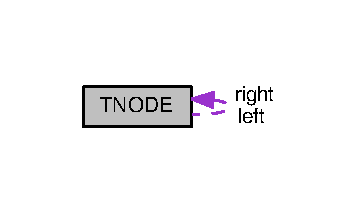
\includegraphics[width=172pt]{structTNODE__coll__graph}
\end{center}
\end{figure}
\subsubsection*{Public Member Functions}
\begin{DoxyCompactItemize}
\item 
\hyperlink{structTNODE_a0f2d73dc28ef3be182dbb07464560a47}{T\+N\+O\+D\+E} ()
\end{DoxyCompactItemize}
\subsubsection*{Public Attributes}
\begin{DoxyCompactItemize}
\item 
char \hyperlink{structTNODE_a436db20d992c4227b8482603b4f76712}{symbol}
\item 
\hyperlink{structTNODE}{T\+N\+O\+D\+E} $\ast$ \hyperlink{structTNODE_ac8548d0ee2d54b914e0e07ab35375dba}{left}
\item 
\hyperlink{structTNODE}{T\+N\+O\+D\+E} $\ast$ \hyperlink{structTNODE_a4e135d9137519b2a4b89dbccb55ae967}{right}
\end{DoxyCompactItemize}


\subsubsection{Constructor \& Destructor Documentation}
\hypertarget{structTNODE_a0f2d73dc28ef3be182dbb07464560a47}{\index{T\+N\+O\+D\+E@{T\+N\+O\+D\+E}!T\+N\+O\+D\+E@{T\+N\+O\+D\+E}}
\index{T\+N\+O\+D\+E@{T\+N\+O\+D\+E}!T\+N\+O\+D\+E@{T\+N\+O\+D\+E}}
\paragraph[{T\+N\+O\+D\+E}]{\setlength{\rightskip}{0pt plus 5cm}T\+N\+O\+D\+E\+::\+T\+N\+O\+D\+E (
\begin{DoxyParamCaption}
{}
\end{DoxyParamCaption}
)\hspace{0.3cm}{\ttfamily [inline]}}}\label{structTNODE_a0f2d73dc28ef3be182dbb07464560a47}

\begin{DoxyCode}
31              \{
32         \hyperlink{structTNODE_a436db20d992c4227b8482603b4f76712}{symbol} = \textcolor{charliteral}{'*'};
33         \hyperlink{structTNODE_ac8548d0ee2d54b914e0e07ab35375dba}{left} = 0;
34         \hyperlink{structTNODE_a4e135d9137519b2a4b89dbccb55ae967}{right} = 0;
35     \}
\end{DoxyCode}


\subsubsection{Member Data Documentation}
\hypertarget{structTNODE_ac8548d0ee2d54b914e0e07ab35375dba}{\index{T\+N\+O\+D\+E@{T\+N\+O\+D\+E}!left@{left}}
\index{left@{left}!T\+N\+O\+D\+E@{T\+N\+O\+D\+E}}
\paragraph[{left}]{\setlength{\rightskip}{0pt plus 5cm}{\bf T\+N\+O\+D\+E}$\ast$ T\+N\+O\+D\+E\+::left}}\label{structTNODE_ac8548d0ee2d54b914e0e07ab35375dba}
\hypertarget{structTNODE_a4e135d9137519b2a4b89dbccb55ae967}{\index{T\+N\+O\+D\+E@{T\+N\+O\+D\+E}!right@{right}}
\index{right@{right}!T\+N\+O\+D\+E@{T\+N\+O\+D\+E}}
\paragraph[{right}]{\setlength{\rightskip}{0pt plus 5cm}{\bf T\+N\+O\+D\+E}$\ast$ T\+N\+O\+D\+E\+::right}}\label{structTNODE_a4e135d9137519b2a4b89dbccb55ae967}
\hypertarget{structTNODE_a436db20d992c4227b8482603b4f76712}{\index{T\+N\+O\+D\+E@{T\+N\+O\+D\+E}!symbol@{symbol}}
\index{symbol@{symbol}!T\+N\+O\+D\+E@{T\+N\+O\+D\+E}}
\paragraph[{symbol}]{\setlength{\rightskip}{0pt plus 5cm}char T\+N\+O\+D\+E\+::symbol}}\label{structTNODE_a436db20d992c4227b8482603b4f76712}


The documentation for this struct was generated from the following file\+:\begin{DoxyCompactItemize}
\item 
\hyperlink{lab_8h}{lab.\+h}\end{DoxyCompactItemize}

\section{File Documentation}
\hypertarget{decode_8cpp}{\subsection{decode.\+cpp File Reference}
\label{decode_8cpp}\index{decode.\+cpp@{decode.\+cpp}}
}
{\ttfamily \#include \char`\"{}lab.\+h\char`\"{}}\\*

\hypertarget{encode_8cpp}{\subsection{encode.\+cpp File Reference}
\label{encode_8cpp}\index{encode.\+cpp@{encode.\+cpp}}
}
{\ttfamily \#include \char`\"{}lab.\+h\char`\"{}}\\*

\hypertarget{lab_8h}{\subsection{lab.\+h File Reference}
\label{lab_8h}\index{lab.\+h@{lab.\+h}}
}
{\ttfamily \#include $<$fstream$>$}\\*
{\ttfamily \#include $<$iostream$>$}\\*
{\ttfamily \#include $<$string$>$}\\*
Include dependency graph for lab.\+h\+:\nopagebreak
\begin{figure}[H]
\begin{center}
\leavevmode
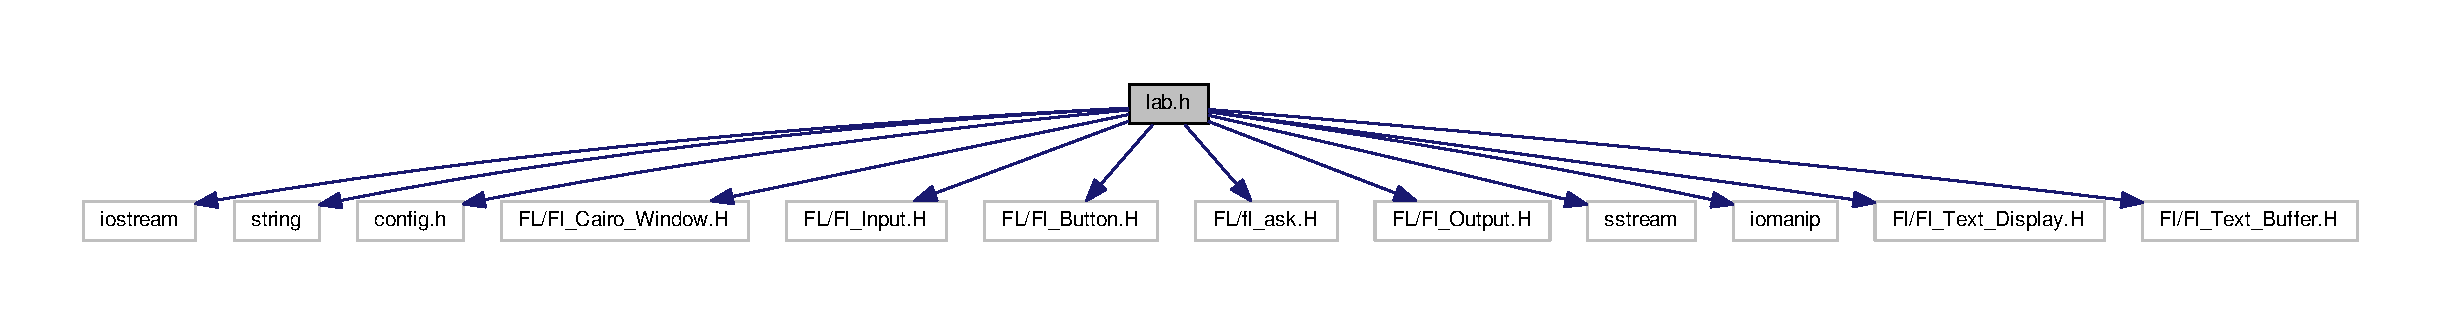
\includegraphics[width=261pt]{lab_8h__incl}
\end{center}
\end{figure}
This graph shows which files directly or indirectly include this file\+:\nopagebreak
\begin{figure}[H]
\begin{center}
\leavevmode
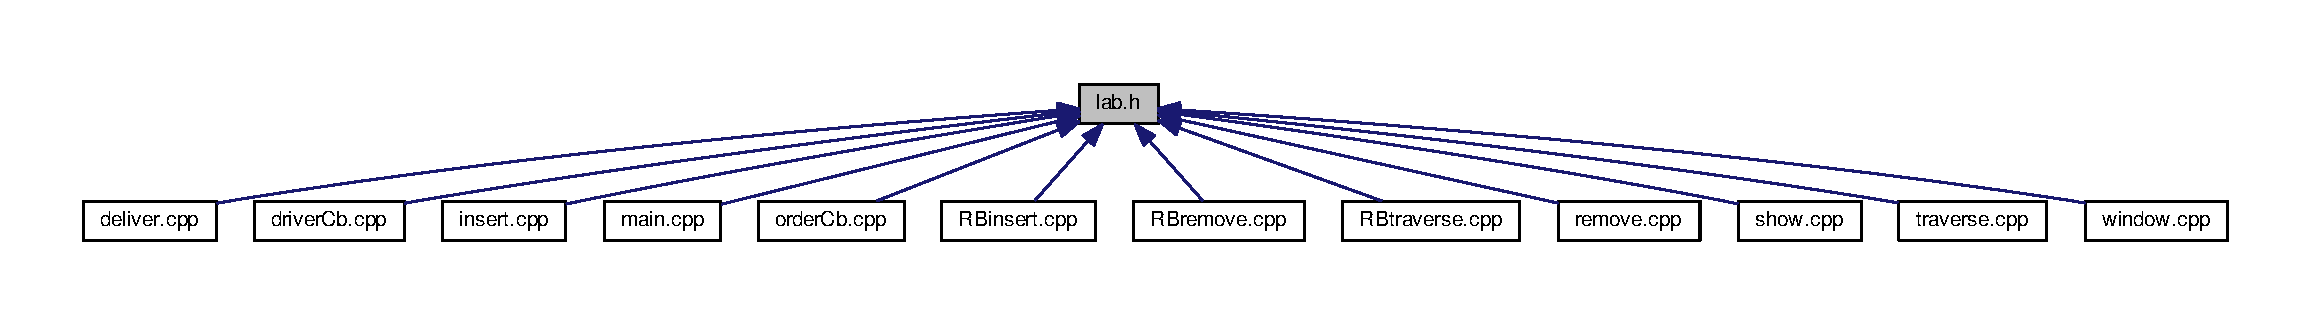
\includegraphics[width=350pt]{lab_8h__dep__incl}
\end{center}
\end{figure}
\subsubsection*{Classes}
\begin{DoxyCompactItemize}
\item 
struct \hyperlink{structNODE}{N\+O\+D\+E}
\begin{DoxyCompactList}\small\item\em City Structure. \end{DoxyCompactList}\end{DoxyCompactItemize}
\subsubsection*{Enumerations}
\begin{DoxyCompactItemize}
\item 
enum \hyperlink{lab_8h_a32c27cc471df37f4fc818d65de0a56c4}{S\+T\+A\+T\+U\+S} \{ \hyperlink{lab_8h_a32c27cc471df37f4fc818d65de0a56c4aecedb56d1405a60c6069f4a0139bdec5}{F\+A\+I\+L\+E\+D}, 
\hyperlink{lab_8h_a32c27cc471df37f4fc818d65de0a56c4a2bc49ec37d6a5715dd23e85f1ff5bb59}{O\+K}
 \}
\end{DoxyCompactItemize}
\subsubsection*{Functions}
\begin{DoxyCompactItemize}
\item 
\hyperlink{lab_8h_a32c27cc471df37f4fc818d65de0a56c4}{S\+T\+A\+T\+U\+S} \hyperlink{lab_8h_a578b73f866dc4391d05ca0219f892495}{insert} (\hyperlink{structNODE}{N\+O\+D\+E} $\ast$\&head, std\+::string city)
\begin{DoxyCompactList}\small\item\em Insert inserts a new node at the beginning of the list. \end{DoxyCompactList}\item 
\hyperlink{lab_8h_a32c27cc471df37f4fc818d65de0a56c4}{S\+T\+A\+T\+U\+S} \hyperlink{lab_8h_abf14767ea6c86eb593d6f87fe77267e7}{insertinorder} (\hyperlink{structNODE}{N\+O\+D\+E} $\ast$\&head, std\+::string city)
\item 
\hyperlink{lab_8h_a32c27cc471df37f4fc818d65de0a56c4}{S\+T\+A\+T\+U\+S} \hyperlink{lab_8h_a9eb7dfa9761b11c255d499765ea70b75}{builddirectly} (\hyperlink{structNODE}{N\+O\+D\+E} $\ast$\&head, string cities)
\item 
void \hyperlink{lab_8h_a67a34562a85e577c0921c5d65c22decc}{destroylist} (\hyperlink{structNODE}{N\+O\+D\+E} $\ast$head)
\item 
void \hyperlink{lab_8h_a6b2cb293574fc5dc8d7a4897cacea16f}{displaylist} (\hyperlink{structNODE}{N\+O\+D\+E} $\ast$head)
\item 
\hyperlink{structNODE}{N\+O\+D\+E} $\ast$ \hyperlink{lab_8h_afd6087490d82489b892a41298eba4e60}{loadlist} (std\+::string filename)
\end{DoxyCompactItemize}


\subsubsection{Enumeration Type Documentation}
\hypertarget{lab_8h_a32c27cc471df37f4fc818d65de0a56c4}{\index{lab.\+h@{lab.\+h}!S\+T\+A\+T\+U\+S@{S\+T\+A\+T\+U\+S}}
\index{S\+T\+A\+T\+U\+S@{S\+T\+A\+T\+U\+S}!lab.\+h@{lab.\+h}}
\paragraph[{S\+T\+A\+T\+U\+S}]{\setlength{\rightskip}{0pt plus 5cm}enum {\bf S\+T\+A\+T\+U\+S}}}\label{lab_8h_a32c27cc471df37f4fc818d65de0a56c4}
\begin{Desc}
\item[Enumerator]\par
\begin{description}
\index{F\+A\+I\+L\+E\+D@{F\+A\+I\+L\+E\+D}!lab.\+h@{lab.\+h}}\index{lab.\+h@{lab.\+h}!F\+A\+I\+L\+E\+D@{F\+A\+I\+L\+E\+D}}\item[{\em 
\hypertarget{lab_8h_a32c27cc471df37f4fc818d65de0a56c4aecedb56d1405a60c6069f4a0139bdec5}{F\+A\+I\+L\+E\+D}\label{lab_8h_a32c27cc471df37f4fc818d65de0a56c4aecedb56d1405a60c6069f4a0139bdec5}
}]\index{O\+K@{O\+K}!lab.\+h@{lab.\+h}}\index{lab.\+h@{lab.\+h}!O\+K@{O\+K}}\item[{\em 
\hypertarget{lab_8h_a32c27cc471df37f4fc818d65de0a56c4a2bc49ec37d6a5715dd23e85f1ff5bb59}{O\+K}\label{lab_8h_a32c27cc471df37f4fc818d65de0a56c4a2bc49ec37d6a5715dd23e85f1ff5bb59}
}]\end{description}
\end{Desc}

\begin{DoxyCode}
7 \{\hyperlink{lab_8h_a32c27cc471df37f4fc818d65de0a56c4aecedb56d1405a60c6069f4a0139bdec5}{FAILED}, \hyperlink{lab_8h_a32c27cc471df37f4fc818d65de0a56c4a2bc49ec37d6a5715dd23e85f1ff5bb59}{OK}\};
\end{DoxyCode}


\subsubsection{Function Documentation}
\hypertarget{lab_8h_a9eb7dfa9761b11c255d499765ea70b75}{\index{lab.\+h@{lab.\+h}!builddirectly@{builddirectly}}
\index{builddirectly@{builddirectly}!lab.\+h@{lab.\+h}}
\paragraph[{builddirectly}]{\setlength{\rightskip}{0pt plus 5cm}{\bf S\+T\+A\+T\+U\+S} builddirectly (
\begin{DoxyParamCaption}
\item[{{\bf N\+O\+D\+E} $\ast$\&}]{head, }
\item[{string}]{cities}
\end{DoxyParamCaption}
)}}\label{lab_8h_a9eb7dfa9761b11c255d499765ea70b75}

\begin{DoxyCode}
5 \{
6     \textcolor{keywordtype}{string} city;
7     \hyperlink{structNODE}{NODE}* tail; 
8     ifstream ifs(\textcolor{stringliteral}{"cities"});
9     \textcolor{keywordflow}{if} (! ifs) 
10     \textcolor{keywordflow}{return} \hyperlink{lab_8h_a32c27cc471df37f4fc818d65de0a56c4aecedb56d1405a60c6069f4a0139bdec5}{FAILED};
11     
12 \textcolor{keywordflow}{while}(ifs >> city) \{
13     \hyperlink{structNODE}{NODE} *newnode = \textcolor{keyword}{new} \hyperlink{structNODE}{NODE};
14     \textcolor{keywordflow}{if}(!newnode)
15     \textcolor{keywordflow}{return} \hyperlink{lab_8h_a32c27cc471df37f4fc818d65de0a56c4aecedb56d1405a60c6069f4a0139bdec5}{FAILED};
16     
17     newnode->\hyperlink{structNODE_a76c9a9603778b363e65bfe84da4bd72e}{city} = city;
18     
19     newnode->\hyperlink{structNODE_a078472e8ab2d2fe38e052f5c2a425618}{next} = 0;
20     
21      \textcolor{keywordflow}{if}(!tail) \{
22         head = newnode;\}
23     \textcolor{keywordflow}{else} \{
24         tail->\hyperlink{structNODE_a078472e8ab2d2fe38e052f5c2a425618}{next} = newnode;
25     \}
26     tail = newnode;
27     
28 \}
29 \}
\end{DoxyCode}
\hypertarget{lab_8h_a67a34562a85e577c0921c5d65c22decc}{\index{lab.\+h@{lab.\+h}!destroylist@{destroylist}}
\index{destroylist@{destroylist}!lab.\+h@{lab.\+h}}
\paragraph[{destroylist}]{\setlength{\rightskip}{0pt plus 5cm}void destroylist (
\begin{DoxyParamCaption}
\item[{{\bf N\+O\+D\+E} $\ast$}]{head}
\end{DoxyParamCaption}
)}}\label{lab_8h_a67a34562a85e577c0921c5d65c22decc}

\begin{DoxyParams}[1]{Parameters}
\mbox{\tt in}  & {\em head} & This is the only parameter the function takes.\\
\hline
\end{DoxyParams}
This function completely destroys the list.


\begin{DoxyImage}
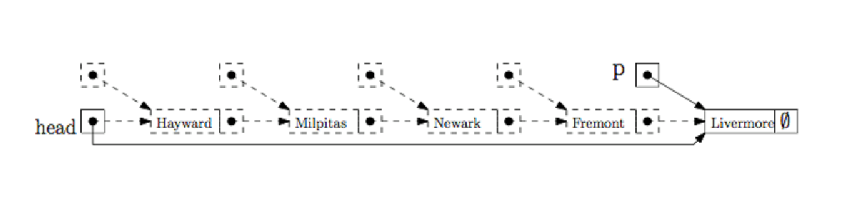
\includegraphics{destroylist1}
\caption{Linked List}
\end{DoxyImage}
 As you can see that this function points the head at the node and then deletes it severing the tie to the list 
\begin{DoxyCode}
14 \{
15     \hyperlink{structNODE}{NODE}* node;
16     \textcolor{keywordflow}{for}(node = head; node; node = node->\hyperlink{structNODE_a078472e8ab2d2fe38e052f5c2a425618}{next})
17     \{
18         cout << \textcolor{stringliteral}{"deleting: "}
19             << node->\hyperlink{structNODE_a76c9a9603778b363e65bfe84da4bd72e}{city} << std::endl;
20         \hyperlink{structNODE}{NODE}* tmp = head->\hyperlink{structNODE_a078472e8ab2d2fe38e052f5c2a425618}{next};
21         \textcolor{keyword}{delete} head;
22         head = tmp;
23         
24     \}
25     
26 \}
\end{DoxyCode}
\hypertarget{lab_8h_a6b2cb293574fc5dc8d7a4897cacea16f}{\index{lab.\+h@{lab.\+h}!displaylist@{displaylist}}
\index{displaylist@{displaylist}!lab.\+h@{lab.\+h}}
\paragraph[{displaylist}]{\setlength{\rightskip}{0pt plus 5cm}void displaylist (
\begin{DoxyParamCaption}
\item[{{\bf N\+O\+D\+E} $\ast$}]{head}
\end{DoxyParamCaption}
)}}\label{lab_8h_a6b2cb293574fc5dc8d7a4897cacea16f}

\begin{DoxyParams}[1]{Parameters}
\mbox{\tt in}  & {\em head} & This fucntion only takes a pointer as an argument.\\
\hline
\end{DoxyParams}
This function displays/traverses the list This is what a linked list looks like to a user It traverses the list without manipulating any pointers. See the comments for further deatils 
\begin{DoxyCode}
11 \{
12     \textcolor{comment}{//first we set the node pointer equal to the head pointer}
13     \textcolor{comment}{//Then while node exists this loop continues}
14     \textcolor{comment}{//Then we set the pointer equal to the next pointer }
15 
16     \textcolor{keywordflow}{for}(\hyperlink{structNODE}{NODE}* node = head; node; node = node->\hyperlink{structNODE_a078472e8ab2d2fe38e052f5c2a425618}{next})
17     \textcolor{comment}{//This displays the data within the node}
18     cout << node->city << endl;
19 \}
\end{DoxyCode}
\hypertarget{lab_8h_a578b73f866dc4391d05ca0219f892495}{\index{lab.\+h@{lab.\+h}!insert@{insert}}
\index{insert@{insert}!lab.\+h@{lab.\+h}}
\paragraph[{insert}]{\setlength{\rightskip}{0pt plus 5cm}{\bf S\+T\+A\+T\+U\+S} insert (
\begin{DoxyParamCaption}
\item[{{\bf N\+O\+D\+E} $\ast$\&}]{head, }
\item[{std\+::string}]{city}
\end{DoxyParamCaption}
)}}\label{lab_8h_a578b73f866dc4391d05ca0219f892495}


Insert inserts a new node at the beginning of the list. 


\begin{DoxyParams}[1]{Parameters}
\mbox{\tt in,out}  & {\em head} & The head of the linked list \\
\hline
\mbox{\tt in}  & {\em city} & The data in the node being inserted \\
\hline
\end{DoxyParams}
\begin{DoxyReturn}{Returns}
A S\+T\+A\+T\+U\+S indicating if Insert was successful of not
\end{DoxyReturn}

\begin{DoxyParams}[1]{Parameters}
\mbox{\tt in,out}  & {\em head} & The head of the linked list \\
\hline
\mbox{\tt in}  & {\em city} & The data in the node being inserted \\
\hline
\end{DoxyParams}
\begin{DoxyReturn}{Returns}
A S\+T\+A\+T\+U\+S indicating if Insert was successful of not 
\begin{DoxyImage}
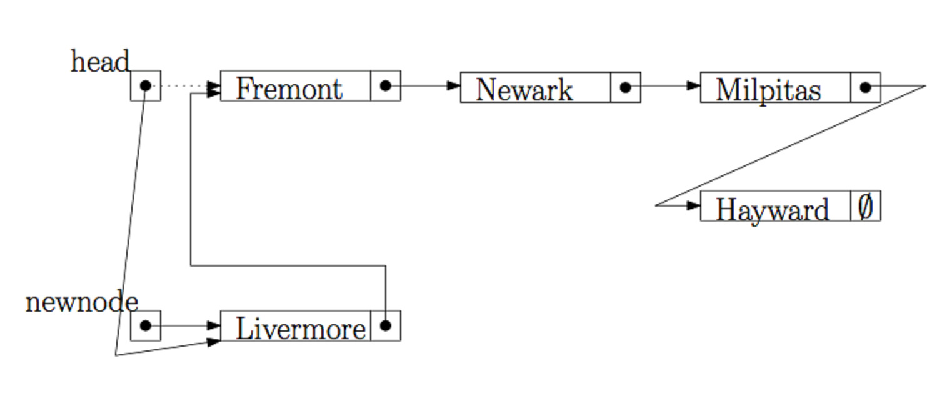
\includegraphics{insert}
\caption{Linked List}
\end{DoxyImage}
 
\end{DoxyReturn}

\begin{DoxyCode}
11 \{
12     \textcolor{comment}{//city = "Dublin"}
13     \hyperlink{structNODE}{NODE} *newnode;
14     
15     \textcolor{comment}{// Allocate a new node:}
16     
17     newnode = \textcolor{keyword}{new} \hyperlink{structNODE}{NODE};
18     \textcolor{keywordflow}{if} (!newnode)
19         \textcolor{keywordflow}{return} \hyperlink{lab_8h_a32c27cc471df37f4fc818d65de0a56c4aecedb56d1405a60c6069f4a0139bdec5}{FAILED}; 
20     \textcolor{comment}{//copy the info into the new node:}
21     
22     newnode->\hyperlink{structNODE_a76c9a9603778b363e65bfe84da4bd72e}{city} = city;
23     
24     \textcolor{comment}{//Link the new node to the list:}
25     
26     newnode->\hyperlink{structNODE_a078472e8ab2d2fe38e052f5c2a425618}{next} = head;
27     head = newnode; 
28     
29     \textcolor{keywordflow}{return} \hyperlink{lab_8h_a32c27cc471df37f4fc818d65de0a56c4a2bc49ec37d6a5715dd23e85f1ff5bb59}{OK}; 
30 \}
\end{DoxyCode}
\hypertarget{lab_8h_abf14767ea6c86eb593d6f87fe77267e7}{\index{lab.\+h@{lab.\+h}!insertinorder@{insertinorder}}
\index{insertinorder@{insertinorder}!lab.\+h@{lab.\+h}}
\paragraph[{insertinorder}]{\setlength{\rightskip}{0pt plus 5cm}{\bf S\+T\+A\+T\+U\+S} insertinorder (
\begin{DoxyParamCaption}
\item[{{\bf N\+O\+D\+E} $\ast$\&}]{head, }
\item[{std\+::string}]{city}
\end{DoxyParamCaption}
)}}\label{lab_8h_abf14767ea6c86eb593d6f87fe77267e7}

\begin{DoxyParams}[1]{Parameters}
\mbox{\tt in}  & {\em head,string} & This functions takes in the head and a string which is whatever city the user defines\\
\hline
\end{DoxyParams}
This function inserts a city into the list in a specific order.


\begin{DoxyImage}
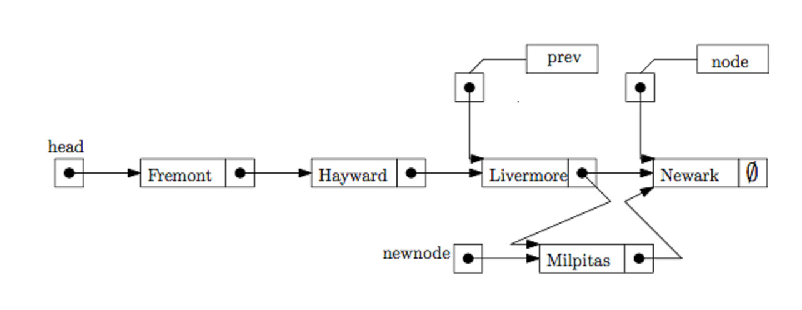
\includegraphics{insertinorder}
\caption{Linked List}
\end{DoxyImage}
 This shows how the pointers previous and next work as they traverse the list looking for a place to insert. Once it does it changes the pointers to add the value into the list 
\begin{DoxyCode}
16 \{
17     \hyperlink{structNODE}{NODE} *newnode;
18      \textcolor{comment}{// Allocate a new node:}
19      
20     newnode = \textcolor{keyword}{new} \hyperlink{structNODE}{NODE};
21     \textcolor{keywordflow}{if} (!newnode)
22         \textcolor{keywordflow}{return} \hyperlink{lab_8h_a32c27cc471df37f4fc818d65de0a56c4aecedb56d1405a60c6069f4a0139bdec5}{FAILED};
23         
24     \textcolor{comment}{// Copy the info into newnode:}
25     
26     newnode->\hyperlink{structNODE_a76c9a9603778b363e65bfe84da4bd72e}{city} = city;
27     
28     \textcolor{comment}{// LINK newnode to the list:}
29     \textcolor{comment}{// a) Find the right place to insert newnode (between "prev" and "node":}
30     
31     \hyperlink{structNODE}{NODE} *\hyperlink{structNODE}{NODE} = head, *prev = 0;
32     \textcolor{keywordflow}{while} (NODE && NODE->\hyperlink{structNODE_a76c9a9603778b363e65bfe84da4bd72e}{city} <= city) \{
33         \textcolor{comment}{//node->city <= city}
34     prev = NODE;        \textcolor{comment}{//advance node and prev}
35     NODE = NODE->\hyperlink{structNODE_a078472e8ab2d2fe38e052f5c2a425618}{next};
36 \}
37     \textcolor{comment}{// b) Link newnode between prev and node}
38     
39     newnode->\hyperlink{structNODE_a078472e8ab2d2fe38e052f5c2a425618}{next} = NODE; \textcolor{comment}{//append node to newnode}
40     \textcolor{keywordflow}{if} (prev)
41         prev->\hyperlink{structNODE_a078472e8ab2d2fe38e052f5c2a425618}{next} = newnode; \textcolor{comment}{//Insert after "prev"}
42     \textcolor{keywordflow}{else} 
43         head = newnode; \textcolor{comment}{//No prev: make new node the new head}
44         
45         \textcolor{keywordflow}{return} \hyperlink{lab_8h_a32c27cc471df37f4fc818d65de0a56c4a2bc49ec37d6a5715dd23e85f1ff5bb59}{OK};
46     \}
\end{DoxyCode}
\hypertarget{lab_8h_afd6087490d82489b892a41298eba4e60}{\index{lab.\+h@{lab.\+h}!loadlist@{loadlist}}
\index{loadlist@{loadlist}!lab.\+h@{lab.\+h}}
\paragraph[{loadlist}]{\setlength{\rightskip}{0pt plus 5cm}{\bf N\+O\+D\+E}$\ast$ loadlist (
\begin{DoxyParamCaption}
\item[{std\+::string}]{filename}
\end{DoxyParamCaption}
)}}\label{lab_8h_afd6087490d82489b892a41298eba4e60}
This function loads the dictionary into a linked list it takes the filename \char`\"{}cities\char`\"{} and loads that as cities the variable Then it uses the insert function to create the list after the head pointer. Then at the end it returns head so that we can use it in other functions. 
\begin{DoxyCode}
10 \{
11     \hyperlink{structNODE}{NODE}* head = 0; \textcolor{comment}{// this is where we declare the head as null to create the list}
12     std::ifstream ifs(filename.c\_str());
13     \textcolor{keywordtype}{string} city;
14     \textcolor{keywordflow}{while}(ifs >> city) 
15         \textcolor{keywordflow}{if}(\hyperlink{insert_8cpp_a578b73f866dc4391d05ca0219f892495}{insert}(head,city) == \hyperlink{lab_8h_a32c27cc471df37f4fc818d65de0a56c4aecedb56d1405a60c6069f4a0139bdec5}{FAILED})
16          cerr << \textcolor{stringliteral}{"error on insert\(\backslash\)n"};
17          
18     \textcolor{keywordflow}{return} head;
19 \}
\end{DoxyCode}

\hypertarget{main_8cpp}{\subsection{main.\+cpp File Reference}
\label{main_8cpp}\index{main.\+cpp@{main.\+cpp}}
}
{\ttfamily \#include \char`\"{}lab.\+h\char`\"{}}\\*
Include dependency graph for main.\+cpp\+:\nopagebreak
\begin{figure}[H]
\begin{center}
\leavevmode
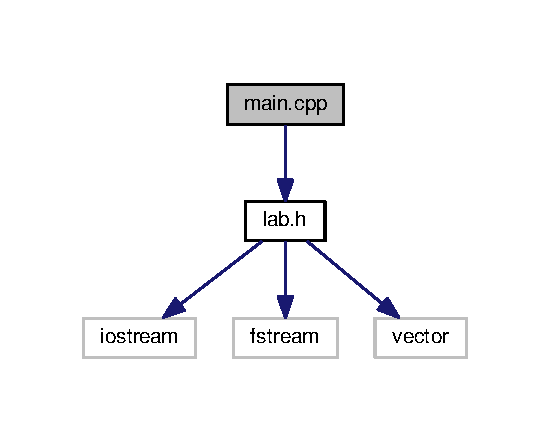
\includegraphics[width=264pt]{main_8cpp__incl}
\end{center}
\end{figure}
\subsubsection*{Functions}
\begin{DoxyCompactItemize}
\item 
int \hyperlink{main_8cpp_ae66f6b31b5ad750f1fe042a706a4e3d4}{main} ()
\end{DoxyCompactItemize}


\subsubsection{Function Documentation}
\hypertarget{main_8cpp_ae66f6b31b5ad750f1fe042a706a4e3d4}{\index{main.\+cpp@{main.\+cpp}!main@{main}}
\index{main@{main}!main.\+cpp@{main.\+cpp}}
\paragraph[{main}]{\setlength{\rightskip}{0pt plus 5cm}int main (
\begin{DoxyParamCaption}
{}
\end{DoxyParamCaption}
)}}\label{main_8cpp_ae66f6b31b5ad750f1fe042a706a4e3d4}
This is main function of the project. Contains the three fucntions (loaddictionary, foundwords, addwords) See comments for better understanding 
\begin{DoxyCode}
11 \{
12     vector<Entry> dict;
13     \textcolor{keywordtype}{string} word; \textcolor{comment}{// user inputs word}
14     \textcolor{keywordtype}{string} translation; \textcolor{comment}{// outputs translation}
15     \textcolor{keywordtype}{bool} ok, quit;
16     
17     ok = \hyperlink{lab_8h_ac18625e34f66c3bc052e07dfb0d3d219}{loaddictionary}(\textcolor{stringliteral}{"dict.dat"}, dict);
18     \textcolor{keywordflow}{if} (!ok) \{
19         cout << \textcolor{stringliteral}{" **** Cannot load Dictionary ***** \(\backslash\)n"};
20         \textcolor{keywordflow}{return} 1; \textcolor{comment}{//ERROR}
21     \}
22     
23     
24     \textcolor{keywordtype}{string} line;
25     
26  ifstream inpfile(\textcolor{stringliteral}{"dict.dat"}); \textcolor{comment}{//opening file again so that once updated }
27     \textcolor{keywordflow}{if} (!inpfile) \textcolor{keywordflow}{return} \textcolor{keyword}{false}; \textcolor{comment}{//the new information can be called without restarting the program}
28     
29     getline(inpfile, line);
30     cout << line << endl;
31     cout << \textcolor{stringliteral}{"Program by Samuel Jothimuthu"} <<endl;
32 
33     quit = \textcolor{keyword}{false};
34     \textcolor{keywordflow}{while} (!quit) \{ \textcolor{comment}{//iteration control structure}
35         \hyperlink{lab_8h_ac18625e34f66c3bc052e07dfb0d3d219}{loaddictionary}(\textcolor{stringliteral}{"dict.dat"}, dict);
36 
37         \textcolor{keywordtype}{string} choice; \textcolor{comment}{//simple choice of yes or no }
38         \textcolor{keywordtype}{string} newtran; \textcolor{comment}{//new translation for word user enters}
39         \textcolor{keywordtype}{string} inputstring; \textcolor{comment}{// the full string that will be appened to the file "dict.dat"}
40         cout << \textcolor{stringliteral}{"Enter a word or 'q' to quit ==> "};
41         cin >> word;
42         cin.ignore(80, \textcolor{charliteral}{'\(\backslash\)n'}); \textcolor{comment}{//this allows the console argument to execute but skipping the line}
43         \textcolor{keywordflow}{if} (word == \textcolor{stringliteral}{"q"}) 
44             quit = \textcolor{keyword}{true};
45         \textcolor{keywordflow}{else} \textcolor{keywordflow}{if} (\hyperlink{foundWord_8cpp_ae41eba27837d0aeea84fb5c6824388db}{foundword}( dict, word, translation)) \textcolor{comment}{//function must return true}
46             cout << translation << \textcolor{stringliteral}{"\(\backslash\)n\(\backslash\)n"};
47         \textcolor{keywordflow}{else} \textcolor{comment}{//The selection control structure}
48            \{ cout << word << \textcolor{stringliteral}{" --not in the dictionary. \(\backslash\)n Would you like to add it? (y/n)\(\backslash\)n"};
49             cin >> choice;
50             \textcolor{keywordflow}{if} (choice == \textcolor{stringliteral}{"y"}) \{ \textcolor{comment}{//any other input does not work. }
51                 cout << \textcolor{stringliteral}{"What is the Italian translation for "} << word << \textcolor{stringliteral}{"?"} << endl;
52                 cin >> newtran;
53                 inputstring = word + \textcolor{stringliteral}{"\(\backslash\)t"} + newtran; \textcolor{comment}{// this builds the full string that the program can
       then call upon.}
54                 \hyperlink{addWords_8cpp_ab5aa985d3bd8d2b89a2d5f35f38fb868}{addwords}(\textcolor{stringliteral}{"dict.dat"}, inputstring); \textcolor{comment}{//runs the addwords function, adding it into the
       file.}
55                 \}
56         \}
57         \}
58         \textcolor{keywordflow}{return} 0;
59     \}
\end{DoxyCode}

\hypertarget{morse_8cpp}{\subsection{morse.\+cpp File Reference}
\label{morse_8cpp}\index{morse.\+cpp@{morse.\+cpp}}
}
{\ttfamily \#include \char`\"{}lab.\+h\char`\"{}}\\*

\hypertarget{morse_8dox}{\subsection{morse.\+dox File Reference}
\label{morse_8dox}\index{morse.\+dox@{morse.\+dox}}
}

%--- End generated contents ---

% Index
\newpage
\phantomsection
\addcontentsline{toc}{section}{Index}
\printindex

\end{document}
